\documentclass[11pt,a4paper]{article}
\usepackage{amsmath}
\usepackage{enumerate}
\usepackage{fancyhdr}
\usepackage{graphicx}
\usepackage{hyperref}
\usepackage[utf8]{inputenc}
\usepackage[a4paper, top=1in, bottom=1.25in, left=0.75in, right=0.75in]{geometry}

\begin{document}
\pagestyle{fancy}
\fancyhead[R]{Niels Hoppe 364399, Robert Schüle 319782, Christoph Ende 331655}

\section*{Connectionist Neurons and Multi Layer Perceptrons}

%%%%%%%%%%%%%%%%%%%%%%%%%%%%%%%%%%%%%%%%%%%%%%%%%%%%%%%%%%%%%%%%%%%%%%%%%%%%%%%%
\subsection*{Terminology}

\begin{enumerate}[a)]
\item

As 3-layered networks with linear transfer functions are equivalent to a single connectionist neuron (p.13), non-linear transfer functions are required achieve the computational capabilities to approximate more complex functions or model more complex behaviour. Basically, we end up with only linear decision boundaries, which might not be sufficient to seperate our data points effectively.

\item

The bias serves as a threshold for the activity signal (p.12). Modifying the threshold moves the decision boundary while preserving it's slope.

In figure 8 of the script (p.8) we see a working example with a bias. If we didn't have a bias, the decision boundary would pass through the origin, making it impossible to reliably distinguish apple-datapoints from orange-datapoints, regardless of it's slope.

\item

Point and edge filters (Sobel filters) are specific linear weights ($w$) for the input vector $x$, used for point and edge detection in images.

\item

The stochastic function has a negative slope at the inflection point and is not deterministic.

\end{enumerate}
%%%%%%%%%%%%%%%%%%%%%%%%%%%%%%%%%%%%%%%%%%%%%%%%%%%%%%%%%%%%%%%%%%%%%%%%%%%%%%%%
\subsection*{Finding Parameters of a Connectionist Neuron}

\begin{enumerate}[a)]
\item
the solutions for this task are stored in the file '2-2.ipynb'

\end{enumerate}
%%%%%%%%%%%%%%%%%%%%%%%%%%%%%%%%%%%%%%%%%%%%%%%%%%%%%%%%%%%%%%%%%%%%%%%%%%%%%%%%
\subsection*{Learning paradigms}

\small{The code for task 3 is stored in '23.py'}
\begin{enumerate}[a)]
\item
Multilayer perceptrons can have several outputs $y_j$, while connectionist neurons only have one output.
The number of outputs defines the maximum amount of classes, that can be distinguished. To distinguish between two classes,
a MLP not only needs two outputs, it also needs to apply two different activation functions. To guarantee that for a MLP with only
one input $x$, the MLP needs at least one hidden layer.\\



\item

Picture \ref{23b} shows 50 simulations of a MLP with ten hidden layers which uses the input-output function \begin{equation} \sum_{i=1}^{n_{hid}}\,w_i\,tanh(a_i(x-b_i)) \end{equation}. The weights $w_i$ were randomly varied between $0$ and $1$,
$a_i$ was randomly varied between $0$ and $2$ and $b_i$ between $-2$ and $2$.
\begin{figure}[h]
  \centering
  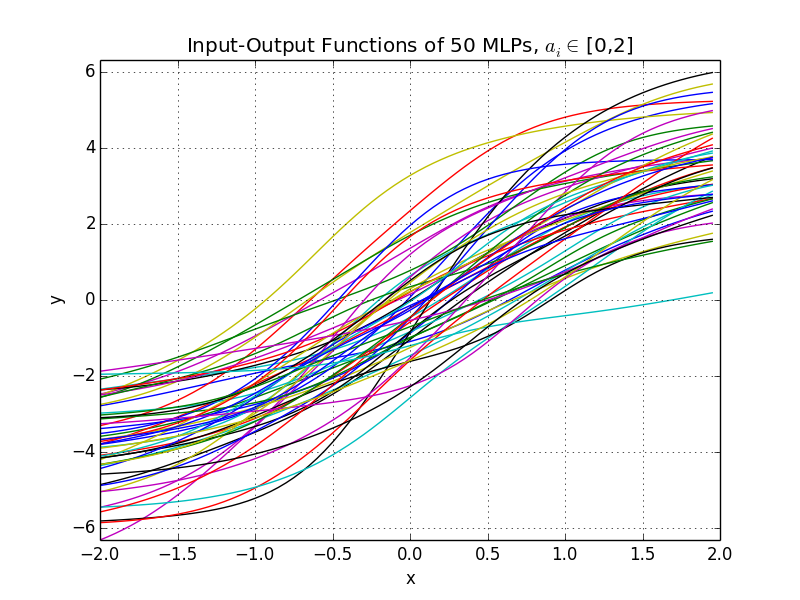
\includegraphics[width=13 cm]{23b.png}
  \caption{Simulation of 2.3 b) }
  \label{23b}
\end{figure}


\item

Now, the maximum value for $a_i$ was reduced from $2$ to $0.5$. This parameter amplifies the argument of the hyperbolic tangent function. Higher values of $a_i$ lead
to a more saturated curve. Since we applied smaller values in this case, the curves appear more linear/ we can see smaller extracts of the hyperbolic tangent function (fig. \ref{23c}).
\begin{figure}[h]
  \centering
  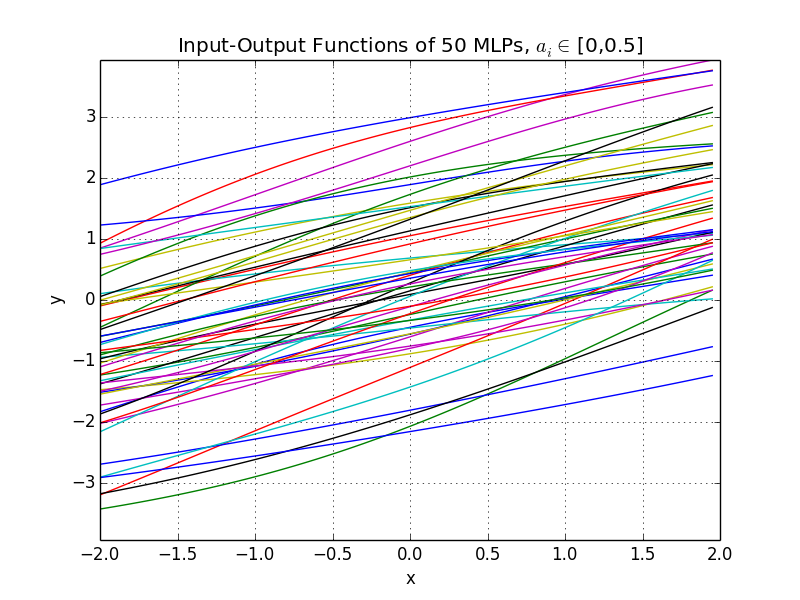
\includegraphics[width=13 cm]{23c.png}
  \caption{Simulation of 2.3 c) }
  \label{23c}
\end{figure}


\end{enumerate}
%%%%%%%%%%%%%%%%%%%%%%%%%%%%%%%%%%%%%%%%%%%%%%%%%%%%%%%%%%%%%%%%%%%%%%%%%%%%%%%%
\end{document}
